\documentclass{article}
\usepackage{tikz}
\usepackage{amsmath}
\begin{document}
	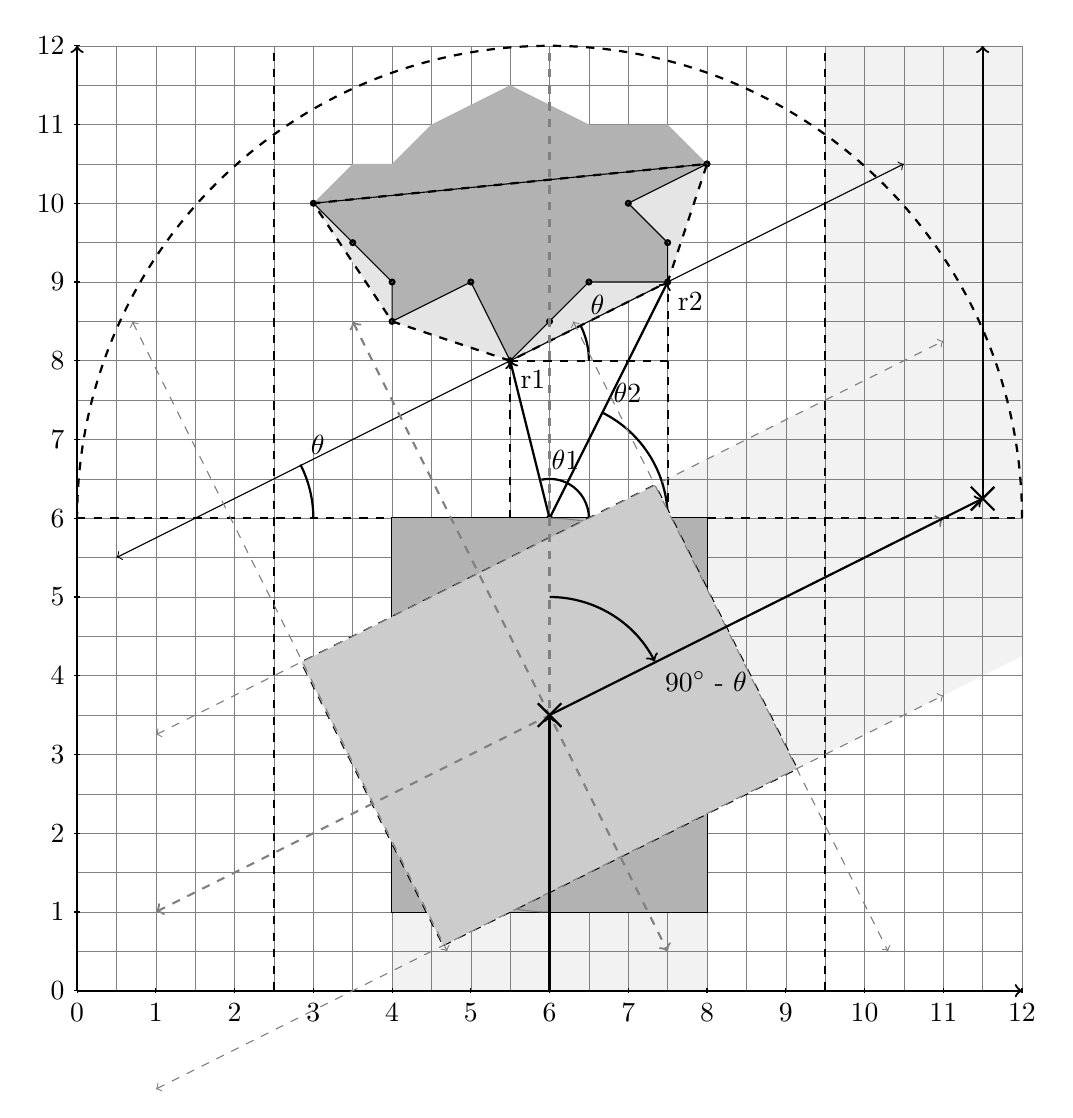
\begin{tikzpicture}
	\fill[black!5!white] (9.14, 2.82) -- (12, 4.25) -- (12, 12) -- (9.5, 12) -- (9.5, 7.5) -- (7.34, 6.42) -- cycle;
	\fill[black!5!white] (4, 0) -- (8, 0) -- (8, 1) -- (4, 1) -- cycle;
	
	\draw[step = 0.5 cm, gray, very thin] (0, 0) grid (12, 12);
	\draw[thick, ->] (0, 0) -- (12, 0);
	\draw[thick, ->] (0, 0) -- (0, 12);
	\foreach \x in {0, ..., 12}
		\draw (\x cm, 1 pt) -- (\x cm, -1 pt) node[anchor = north] {$\x$};
	\foreach \y in {0, ..., 12}
		\draw (1 pt, \y cm) -- (-1 pt, \y cm) node[anchor = east] {$\y$};	
	
	\fill[black!10!white] (4, 8.5) -- (5.5, 8) -- (7.5, 9) -- (8, 10.5) -- (3, 10) -- cycle;
	
	\fill[black!30!white] (4, 8.5) -- (5, 9) -- (5.5, 8) -- (6, 8.5) -- (6.5, 9) -- (7.5, 9) -- (7.5, 9.5) -- (7, 10) -- (8, 10.5) -- (7.5, 11) -- (6.5, 11) -- (5.5, 11.5) -- (4.5, 11) -- (4, 10.5) -- (3.5, 10.5) -- (3, 10) -- (3.5, 9.5) -- (4, 9) -- cycle;
	
	\draw[thick, dashed] (4, 8.5) -- (5.5, 8) -- (7.5, 9) -- (8, 10.5) -- (3, 10) -- cycle;
	
	\draw[thick] (4, 8.5) circle (0.03 cm);
	\draw[thick] (5.5, 8) circle (0.03 cm);
	\draw[thick] (7.5, 9) circle (0.03 cm);
	\draw[thick] (8, 10.5) circle (0.03 cm);
	\draw[thick] (3, 10) circle (0.03 cm);
	\draw[thick] (3.5, 9.5) circle (0.03 cm);
	\draw[thick] (4, 9) circle (0.03 cm);
	\draw[thick] (5, 9) circle (0.03 cm);
	\draw[thick] (6, 8.5) circle (0.03 cm);
	\draw[thick] (6.5, 9) circle (0.03 cm);
	\draw[thick] (7.5, 9.5) circle (0.03 cm);
	\draw[thick] (7, 10) circle (0.03 cm);
	
	\draw[thin] (4, 8.5) -- (5, 9) -- (5.5, 8) -- (6, 8.5) -- (6.5, 9) -- (7.5, 9) -- (7.5, 9.5) -- (7, 10) -- (8, 10.5) -- (3, 10) -- (3.5, 9.5) -- (4, 9) -- cycle;
	
	\draw[<->] (0.5, 5.5) -- (10.5, 10.5);
	\draw[thick] (3, 6) arc (0:27:1.5) node[anchor = south west] {$\theta$};
	
	\draw[thick, dashed] (12, 6) arc (0: 180: 6); 
	\draw[thick, dashed] (2.5, 0) -- (2.5, 12);
	\draw[thick, dashed] (9.5, 0) -- (9.5, 12);
	\draw[thick, dashed] (0, 6) -- (12, 6);
	
	\draw[thick] (4, 1) -- (8, 1) -- (8, 6) -- (4, 6) -- cycle;
	\draw[thick] (6, 6) circle (0.03 cm);
	\fill[black!30!white] (4, 1) rectangle (8, 6);
	
	\draw[thick, ->] (6, 6) -- (5.5, 8) node[anchor = north west] {r1};
	\draw[thick] (6.5, 6) arc (0:102:0.5) node[anchor = south west] {$\theta$1};
	
	\draw[thick, ->] (6, 6) -- (7.5, 9) node[anchor = north west] {r2};
	\draw[thick] (7.5, 6) arc (0:63:1.5) node[anchor = south west] {$\theta$2};
	
	\draw[thick, dashed] (5.5, 8) -- (7.5, 8);
	\draw[thick, dashed] (5.5, 6) -- (5.5, 8);
	\draw[thick, dashed] (7.5, 6) -- (7.5, 9);
	\draw[thick] (6.5, 8) arc (0:27:1) node[anchor = south west] {$\theta$};
	
	\draw[gray, thin] (4, 3.5) arc (180:90:2);
	\draw[gray, thin] (8, 3.5) arc (0:-90:2);
	\draw[gray, thin] (8.5, 3.5) arc (0:90:2.5);
	\draw[gray, thin] (6, 1) arc (270:180:2.5);
	
	\draw[thick, dashed] (4.65, 0.58) -- (9.14, 2.82) -- (7.34, 6.42) -- (2.85, 4.17) -- cycle;
	\fill[black!20!white] (4.65, 0.58) -- (9.14, 2.82) -- (7.34, 6.42) -- (2.85, 4.17) -- cycle;
	
	\draw[gray, thick, dashed, <->] (1, 1) -- (11, 6);
	\draw[gray, thick, dashed, <->] (3.5, 8.5) -- (7.5, 0.5);
	
	\draw[gray, thin, dashed, <->] (6.3, 8.5) -- (10.3, 0.5);
	\draw[gray, thin, dashed, <->] (0.7, 8.5) -- (4.7, 0.5);
	\draw[gray, thin, dashed, <->] (1, 3.25) -- (11, 8.25);
	\draw[gray, thin, dashed, <->] (1, -1.25) -- (11, 3.75);
	
	\draw[gray, thick, dashed] (6, 0) -- (6, 12);
	
	\draw[thick] (5.85, 3.35) -- (6.15, 3.65);
	\draw[thick] (5.85, 3.65) -- (6.15, 3.35);
	
	\draw[thick, ->] (6, 5) arc (90:27:1.5) node [anchor =  north west] {$90^{\circ}$ - $\theta$};
	
	\draw[thick] (11.35, 6.1) -- (11.65, 6.4);
	\draw[thick] (11.35, 6.4) -- (11.65, 6.1);
	
	\draw[thick, ->] (6, 3.5) -- (11.5, 6.25);
	\draw[thick, ->] (6, 0) -- (6, 3.5);
	\draw[thick, ->] (11.5, 6.25) -- (11.5, 12);
	\end{tikzpicture}
	
	\begin{align}
	\tan{\theta} & = \frac{h_{2} - h_{1}}{w_{2} - w_{1}} \\
	&= \frac{r_{2} \cos{\theta_{2}} - r_{1} \cos{\theta_{1}}}{r_{2} \sin{\theta_{2}} - r_{1} \sin{\theta_{1}}} \\
	\theta & = \arctan{\frac{r_{2} \cos{\theta_{2}} - r_{1} \cos{\theta_{1}}}{r_{2} \sin{\theta_{2}} - r_{1} \sin{\theta_{1}}}} \\
	\alpha & = 90^{\circ} - \theta \\
	& = \arctan{\frac{r_{2} \sin{\theta_{2}} - r_{1} \sin{\theta_{1}}}{r_{2} \cos{\theta_{2}} - r_{1} \cos{\theta_{1}}}}
	\end{align}
	
	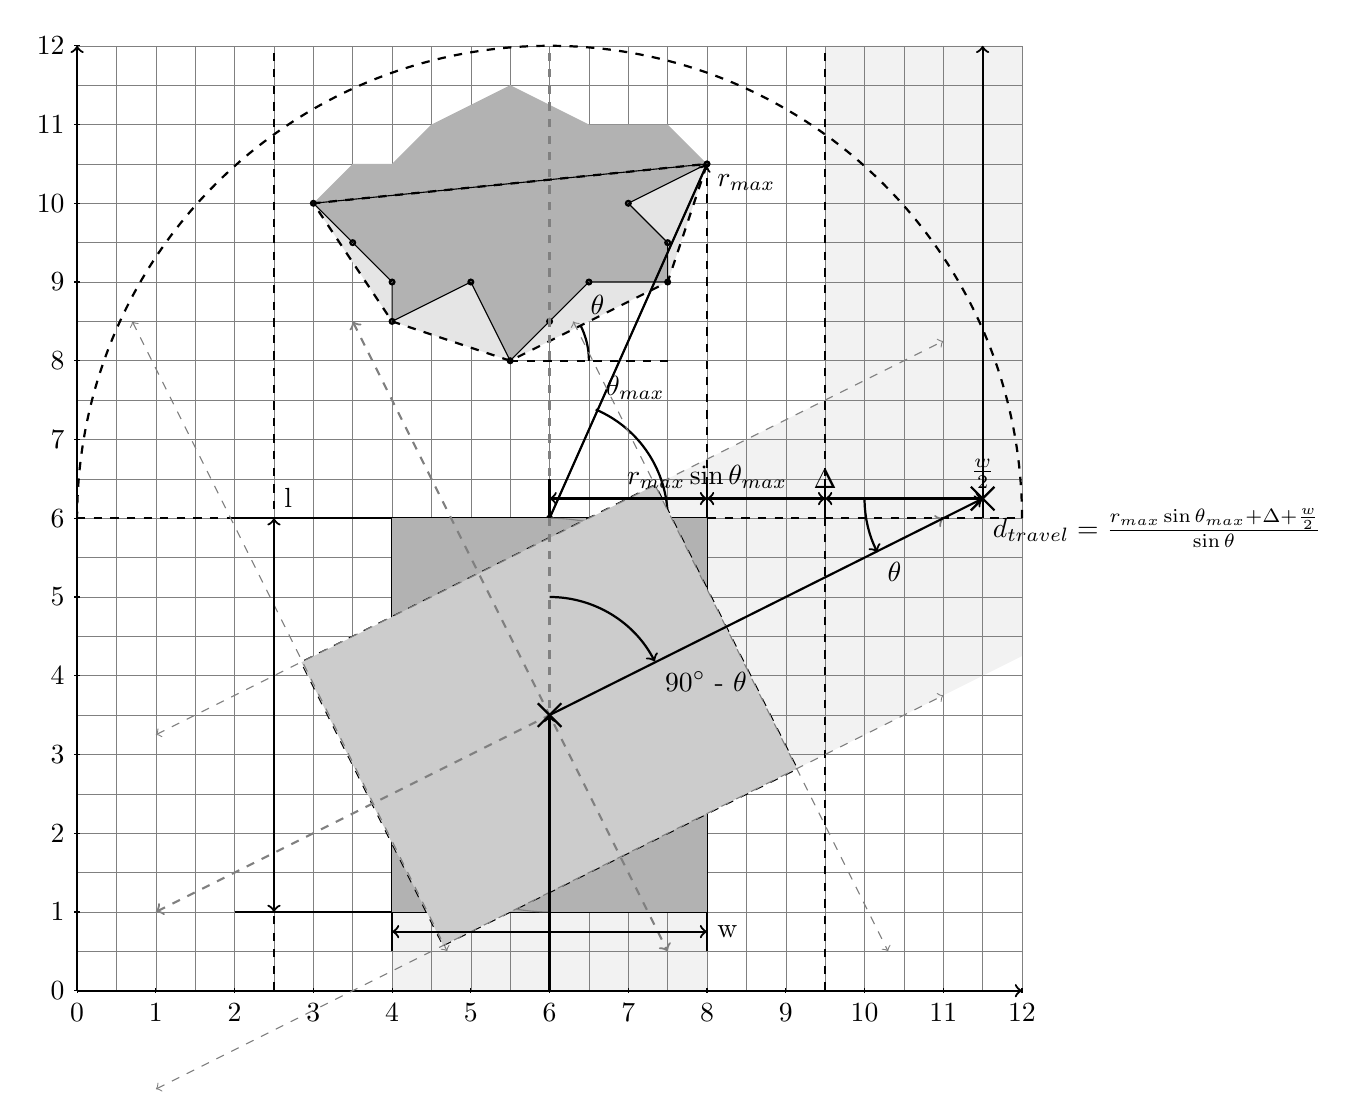
\begin{tikzpicture}
	\fill[black!5!white] (9.14, 2.82) -- (12, 4.25) -- (12, 12) -- (9.5, 12) -- (9.5, 7.5) -- (7.34, 6.42) -- cycle;
	\fill[black!5!white] (4, 0) -- (8, 0) -- (8, 1) -- (4, 1) -- cycle;
	
	\draw[step = 0.5 cm, gray, very thin] (0, 0) grid (12, 12);
	\draw[thick, ->] (0, 0) -- (12, 0);
	\draw[thick, ->] (0, 0) -- (0, 12);
	\foreach \x in {0, ..., 12}
	\draw (\x cm, 1 pt) -- (\x cm, -1 pt) node[anchor = north] {$\x$};
	\foreach \y in {0, ..., 12}
	\draw (1 pt, \y cm) -- (-1 pt, \y cm) node[anchor = east] {$\y$};	
	
	\fill[black!10!white] (4, 8.5) -- (5.5, 8) -- (7.5, 9) -- (8, 10.5) -- (3, 10) -- cycle;
	
	\fill[black!30!white] (4, 8.5) -- (5, 9) -- (5.5, 8) -- (6, 8.5) -- (6.5, 9) -- (7.5, 9) -- (7.5, 9.5) -- (7, 10) -- (8, 10.5) -- (7.5, 11) -- (6.5, 11) -- (5.5, 11.5) -- (4.5, 11) -- (4, 10.5) -- (3.5, 10.5) -- (3, 10) -- (3.5, 9.5) -- (4, 9) -- cycle;
	
	\draw[thick, dashed] (4, 8.5) -- (5.5, 8) -- (7.5, 9) -- (8, 10.5) -- (3, 10) -- cycle;
	
	\draw[thick] (4, 8.5) circle (0.03 cm);
	\draw[thick] (5.5, 8) circle (0.03 cm);
	\draw[thick] (7.5, 9) circle (0.03 cm);
	\draw[thick] (8, 10.5) circle (0.03 cm);
	\draw[thick] (3, 10) circle (0.03 cm);
	\draw[thick] (3.5, 9.5) circle (0.03 cm);
	\draw[thick] (4, 9) circle (0.03 cm);
	\draw[thick] (5, 9) circle (0.03 cm);
	\draw[thick] (6, 8.5) circle (0.03 cm);
	\draw[thick] (6.5, 9) circle (0.03 cm);
	\draw[thick] (7.5, 9.5) circle (0.03 cm);
	\draw[thick] (7, 10) circle (0.03 cm);
	
	\draw[thin] (4, 8.5) -- (5, 9) -- (5.5, 8) -- (6, 8.5) -- (6.5, 9) -- (7.5, 9) -- (7.5, 9.5) -- (7, 10) -- (8, 10.5) -- (3, 10) -- (3.5, 9.5) -- (4, 9) -- cycle;
	
	\draw[thick, dashed] (12, 6) arc (0: 180: 6); 
	\draw[thick, dashed] (2.5, 0) -- (2.5, 12);
	\draw[thick, dashed] (9.5, 0) -- (9.5, 12);
	\draw[thick, dashed] (0, 6) -- (12, 6);
	
	\draw[thick] (4, 1) -- (8, 1) -- (8, 6) -- (4, 6) -- cycle;
	\draw[thick] (6, 6) circle (0.03 cm);
	\fill[black!30!white] (4, 1) rectangle (8, 6);
	
	\draw[thick, ->] (6, 6) -- (8, 10.5) node[anchor = north west] {$r_{max}$};
	\draw[thick] (7.5, 6) arc (0:67:1.5) node[anchor = south west] {$\theta_{max}$};
	
	\draw[thick, dashed] (5.5, 8) -- (7.5, 8);
	\draw[thick, dashed] (8, 6) -- (8, 10.5);
	\draw[thick] (6.5, 8) arc (0:27:1) node[anchor = south west] {$\theta$};
	
	\draw[gray, thin] (4, 3.5) arc (180:90:2);
	\draw[gray, thin] (8, 3.5) arc (0:-90:2);
	\draw[gray, thin] (8.5, 3.5) arc (0:90:2.5);
	\draw[gray, thin] (6, 1) arc (270:180:2.5);
	
	\draw[thick, dashed] (4.65, 0.58) -- (9.14, 2.82) -- (7.34, 6.42) -- (2.85, 4.17) -- cycle;
	\fill[black!20!white] (4.65, 0.58) -- (9.14, 2.82) -- (7.34, 6.42) -- (2.85, 4.17) -- cycle;
	
	\draw[gray, thick, dashed, <->] (1, 1) -- (11, 6);
	\draw[gray, thick, dashed, <->] (3.5, 8.5) -- (7.5, 0.5);
	
	\draw[gray, thin, dashed, <->] (6.3, 8.5) -- (10.3, 0.5);
	\draw[gray, thin, dashed, <->] (0.7, 8.5) -- (4.7, 0.5);
	\draw[gray, thin, dashed, <->] (1, 3.25) -- (11, 8.25);
	\draw[gray, thin, dashed, <->] (1, -1.25) -- (11, 3.75);
	
	\draw[gray, thick, dashed] (6, 0) -- (6, 12);
	
	\draw[thick] (5.85, 3.35) -- (6.15, 3.65);
	\draw[thick] (5.85, 3.65) -- (6.15, 3.35);
	
	\draw[thick, ->] (6, 5) arc (90:27:1.5) node [anchor =  north west] {$90^{\circ}$ - $\theta$};
	
	\draw[thick] (11.35, 6.1) -- (11.65, 6.4);
	\draw[thick] (11.35, 6.4) -- (11.65, 6.1);
	
	\draw[thick, ->] (6, 3.5) -- (11.5, 6.25) node[anchor= north west] {$d_{travel} = \frac{r_{max}\sin{\theta_{max}} + \Delta + \frac{w}{2}}{\sin{\theta}}$};
	
	\draw[thick, ->] (6, 0) -- (6, 3.5);
	\draw[thick, ->] (11.5, 6.25) -- (11.5, 12);
	
	\draw[thick] (6, 6) -- (6, 6.5);
	\draw[thick, <->] (6, 6.25) -- (8, 6.25) node[anchor = south] {$r_{max}\sin{\theta_{max}}$};	
	\draw[thick] (8, 6) -- (8, 6.5);
	\draw[thick] (9.5, 6) -- (9.5, 6.5);
	\draw[thick, <->] (8, 6.25) -- (9.5, 6.25) node[anchor = south] {$\Delta$};
	
	\draw[thick] (11.5, 6) -- (11.5, 6.5);
	\draw[thick, <->] (9.5, 6.25) -- (11.5, 6.25) node[anchor = south] {$\frac{w}{2}$};
	
	\draw[thick, ->] (10, 6.25) arc (180:207:1.5) node [anchor =  north west] {$\theta$};
	
	\draw[thick] (2, 1) -- (4, 1);
	\draw[thick] (2, 6) -- (4, 6);
	\draw[thick, <->] (2.5, 1) -- (2.5, 6) node[anchor = south west] {l};
	
	\draw[thick] (4, 0.5) -- (4, 1);
	\draw[thick] (8, 0.5) -- (8, 1);
	\draw[thick, <->] (4, 0.75) -- (8, 0.75) node[anchor = west] {w};
	\end{tikzpicture}
	
	\begin{align}
	d_{travel} \sin{\theta} &= r_{max}\sin{\theta_{max}} + \Delta + \frac{w}{2} \\
	d_{travel} &= \frac{r_{max}\sin{\theta_{max}} + \Delta + \frac{w}{2}}{\sin{\theta}}
	\end{align}
	
	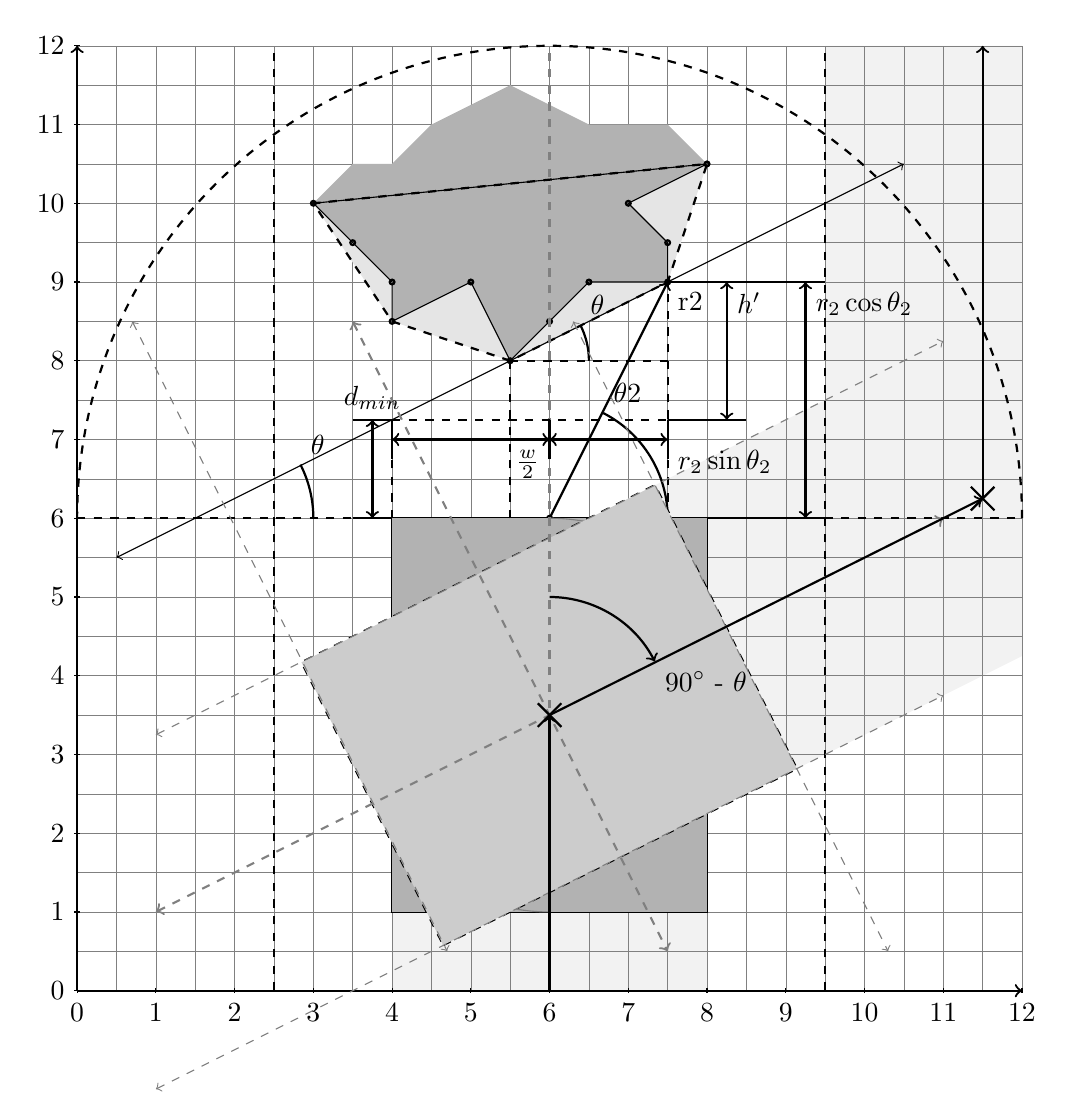
\begin{tikzpicture}
	\fill[black!5!white] (9.14, 2.82) -- (12, 4.25) -- (12, 12) -- (9.5, 12) -- (9.5, 7.5) -- (7.34, 6.42) -- cycle;
	\fill[black!5!white] (4, 0) -- (8, 0) -- (8, 1) -- (4, 1) -- cycle;
	
	\draw[step = 0.5 cm, gray, very thin] (0, 0) grid (12, 12);
	\draw[thick, ->] (0, 0) -- (12, 0);
	\draw[thick, ->] (0, 0) -- (0, 12);
	\foreach \x in {0, ..., 12}
	\draw (\x cm, 1 pt) -- (\x cm, -1 pt) node[anchor = north] {$\x$};
	\foreach \y in {0, ..., 12}
	\draw (1 pt, \y cm) -- (-1 pt, \y cm) node[anchor = east] {$\y$};	
	
	\fill[black!10!white] (4, 8.5) -- (5.5, 8) -- (7.5, 9) -- (8, 10.5) -- (3, 10) -- cycle;
	
	\fill[black!30!white] (4, 8.5) -- (5, 9) -- (5.5, 8) -- (6, 8.5) -- (6.5, 9) -- (7.5, 9) -- (7.5, 9.5) -- (7, 10) -- (8, 10.5) -- (7.5, 11) -- (6.5, 11) -- (5.5, 11.5) -- (4.5, 11) -- (4, 10.5) -- (3.5, 10.5) -- (3, 10) -- (3.5, 9.5) -- (4, 9) -- cycle;
	
	\draw[thick, dashed] (4, 8.5) -- (5.5, 8) -- (7.5, 9) -- (8, 10.5) -- (3, 10) -- cycle;
	
	\draw[thick] (4, 8.5) circle (0.03 cm);
	\draw[thick] (5.5, 8) circle (0.03 cm);
	\draw[thick] (7.5, 9) circle (0.03 cm);
	\draw[thick] (8, 10.5) circle (0.03 cm);
	\draw[thick] (3, 10) circle (0.03 cm);
	\draw[thick] (3.5, 9.5) circle (0.03 cm);
	\draw[thick] (4, 9) circle (0.03 cm);
	\draw[thick] (5, 9) circle (0.03 cm);
	\draw[thick] (6, 8.5) circle (0.03 cm);
	\draw[thick] (6.5, 9) circle (0.03 cm);
	\draw[thick] (7.5, 9.5) circle (0.03 cm);
	\draw[thick] (7, 10) circle (0.03 cm);
	
	\draw[thin] (4, 8.5) -- (5, 9) -- (5.5, 8) -- (6, 8.5) -- (6.5, 9) -- (7.5, 9) -- (7.5, 9.5) -- (7, 10) -- (8, 10.5) -- (3, 10) -- (3.5, 9.5) -- (4, 9) -- cycle;
	
	\draw[<->] (0.5, 5.5) -- (10.5, 10.5);
	\draw[thick] (3, 6) arc (0:27:1.5) node[anchor = south west] {$\theta$};
	
	\draw[thick, dashed] (12, 6) arc (0: 180: 6); 
	\draw[thick, dashed] (2.5, 0) -- (2.5, 12);
	\draw[thick, dashed] (9.5, 0) -- (9.5, 12);
	\draw[thick, dashed] (0, 6) -- (12, 6);
	
	\draw[thick] (4, 1) -- (8, 1) -- (8, 6) -- (4, 6) -- cycle;
	\draw[thick] (6, 6) circle (0.03 cm);
	\fill[black!30!white] (4, 1) rectangle (8, 6);
	
	\draw[thick, ->] (6, 6) -- (7.5, 9) node[anchor = north west] {r2};
	\draw[thick] (7.5, 6) arc (0:63:1.5) node[anchor = south west] {$\theta$2};
	
	\draw[thick, dashed] (5.5, 8) -- (7.5, 8);
	\draw[thick, dashed] (5.5, 6) -- (5.5, 8);
	\draw[thick, dashed] (7.5, 6) -- (7.5, 9);
	\draw[thick] (6.5, 8) arc (0:27:1) node[anchor = south west] {$\theta$};
	
	\draw[gray, thin] (4, 3.5) arc (180:90:2);
	\draw[gray, thin] (8, 3.5) arc (0:-90:2);
	\draw[gray, thin] (8.5, 3.5) arc (0:90:2.5);
	\draw[gray, thin] (6, 1) arc (270:180:2.5);
	
	\draw[thick, dashed] (4.65, 0.58) -- (9.14, 2.82) -- (7.34, 6.42) -- (2.85, 4.17) -- cycle;
	\fill[black!20!white] (4.65, 0.58) -- (9.14, 2.82) -- (7.34, 6.42) -- (2.85, 4.17) -- cycle;
	
	\draw[gray, thick, dashed, <->] (1, 1) -- (11, 6);
	\draw[gray, thick, dashed, <->] (3.5, 8.5) -- (7.5, 0.5);
	
	\draw[gray, thin, dashed, <->] (6.3, 8.5) -- (10.3, 0.5);
	\draw[gray, thin, dashed, <->] (0.7, 8.5) -- (4.7, 0.5);
	\draw[gray, thin, dashed, <->] (1, 3.25) -- (11, 8.25);
	\draw[gray, thin, dashed, <->] (1, -1.25) -- (11, 3.75);
	
	\draw[gray, thick, dashed] (6, 0) -- (6, 12);
	
	\draw[thick] (5.85, 3.35) -- (6.15, 3.65);
	\draw[thick] (5.85, 3.65) -- (6.15, 3.35);
	
	\draw[thick, ->] (6, 5) arc (90:27:1.5) node [anchor =  north west] {$90^{\circ}$ - $\theta$};
	
	\draw[thick] (11.35, 6.1) -- (11.65, 6.4);
	\draw[thick] (11.35, 6.4) -- (11.65, 6.1);
	
	\draw[thick, ->] (6, 3.5) -- (11.5, 6.25);
	\draw[thick, ->] (6, 0) -- (6, 3.5);
	\draw[thick, ->] (11.5, 6.25) -- (11.5, 12);
	
	\draw[thick, dashed] (4, 6) -- (4, 7.25);
	\draw[thick] (3.5, 6) -- (4, 6);
	\draw[thick] (3.5, 7.25) -- (4, 7.25);
	\draw[thick, <->] (3.75, 6) -- (3.75, 7.25) node[anchor = south] {$d_{min}$};
	
	\draw[thick, dashed] (4, 7.25) -- (7.5, 7.25);
	\draw[thick] (4, 6.75) -- (4, 7.25);
	\draw[thick] (6, 6.75) -- (6, 7.25);
	\draw[thick, <->] (4, 7) -- (6, 7) node[anchor = north east] {$\frac{w}{2}$};
	
	\draw[thick] (7.5, 6.75) -- (7.5, 7.25);
	\draw[thick, <->] (6, 7) -- (7.5, 7) node[anchor = north west] {$r_{2} \sin{\theta_{2}}$};
	
	\draw[thick] (7.5, 7.25) -- (8.5, 7.25);
	\draw[thick] (7.5, 9) -- (9.5, 9);
	\draw[thick, <->] (8.25, 7.25) -- (8.25, 9) node[anchor = north west] {$h^{\prime}$};
	\draw[thick] (8, 6) -- (9.5, 6);
	\draw[thick, <->] (9.25, 6) -- (9.25, 9) node[anchor = north west] {$r_{2} \cos{\theta_{2}}$};
	\end{tikzpicture}
	
	\begin{align}
	h^{\prime} &= \left(\frac{w}{2} + r_{2} \sin{\theta_{2}}\right) \tan{\theta} \\
	d_{min} &= r_{2} \cos{\theta_{2}} - h^{\prime} \\
	&= r_{2} \cos{\theta_{2}} - \left(\frac{w}{2} + r_{2} \sin{\theta_{2}}\right) \tan{\theta} \\
	&= r_{2} \cos{\theta_{2}} - \left(\frac{w}{2}\right) \tan{\theta} - r_{2} \sin{\theta_{2}} \tan{\theta} \\
	&= r_{2} \cos{\theta_{2}} - r_{2} \sin{\theta_{2}} \left(\frac{\sin{\theta}}{\cos{\theta}}\right) - \left(\frac{w}{2}\right) \tan{\theta} \\
	&= \frac{r_{2}}{\cos{\theta}} \left(\cos{\theta_{2}} \cos{\theta} - \sin{\theta_{2}} \sin{\theta}\right) - \left(\frac{w}{2}\right) \tan{\theta} \\
	&= \left(\frac{r_{2}}{\cos{\theta}}\right) \cos{\left(\theta_{2} + \theta\right)} - \left(\frac{w}{2}\right) \tan{\theta} \\
	d_{min} &= \left(r_{2} \cos{\left(\theta_{2} + \theta\right)} - \left(\frac{w}{2}\right) \sin{\theta}\right) \frac{1}{\cos{\theta}}
	\end{align}
	
	\begin{align}
	d_{min} &\ge \Delta_{min}
	\end{align}
	
	\begin{align}
	t_{hit} &= \frac{d_{min}}{v_{robo}} \\
	\implies t_{decision} &\le t_{hit}
	\end{align}
	
	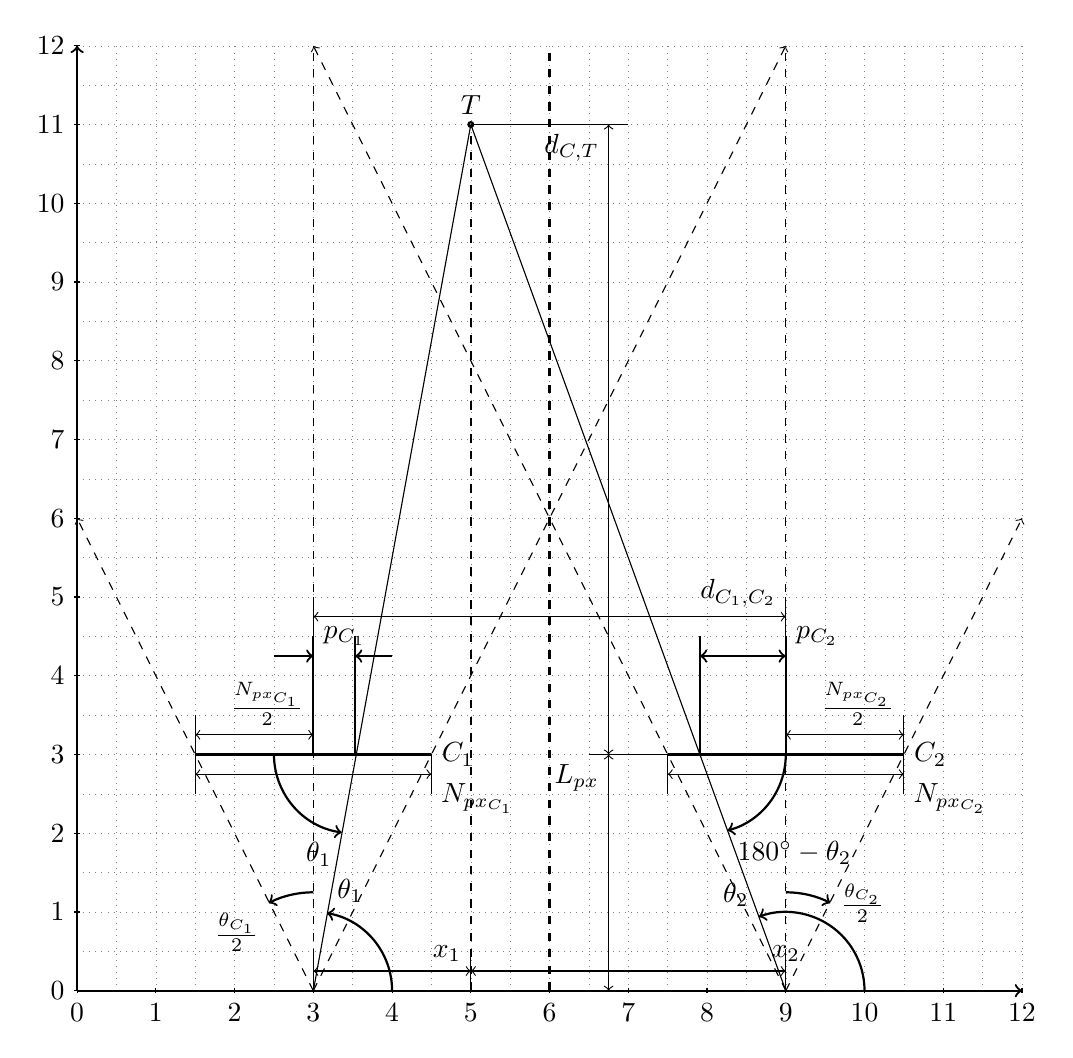
\begin{tikzpicture}
		\draw[step = 0.5 cm, gray, very thin, dotted] (0, 0) grid (12, 12);
		\draw[thick, ->] (0, 0) -- (12, 0);
		\draw[thick, ->] (0, 0) -- (0, 12);
		\foreach \x in {0, ..., 12}
		\draw (\x cm, 1 pt) -- (\x cm, -1 pt) node[anchor = north] {$\x$};
		\foreach \y in {0, ..., 12}
		\draw (1 pt, \y cm) -- (-1 pt, \y cm) node[anchor = east] {$\y$};	
		
		\draw[thick, dashed] (6, 0) -- (6, 12);
		
		\draw[thin, dashed, ->] (3, 0) -- (0, 6);
		\draw[thin, dashed, ->] (3, 0) -- (9, 12);
		\draw[thin, dashed] (3, 0) -- (3, 12);
		
		\draw[thin, dashed, ->] (9, 0) -- (3, 12);
		\draw[thin, dashed, ->] (9, 0) -- (12, 6);
		\draw[thin, dashed] (9, 0) -- (9, 12);
		
		\draw[thick] (5, 11) circle (0.03 cm) node[anchor = south] {$T$};
		
		\draw[thick] (1.5, 3) -- (4.5, 3) node [anchor = west] {$C_{1}$};
		
		\draw[thick] (7.5, 3) -- (10.5, 3) node [anchor = west] {$C_{2}$};;
		
		\draw[thin] (3, 0) -- (5, 11);
		\draw[thin] (5, 11) -- (9, 0);
		
		\draw[thick, dashed] (5, 0) -- (5, 11);
		
		\draw [thick] (3, 3) -- (3, 4.5);
		\draw [thick] (3.53, 3) -- (3.53, 4.5);
		\draw [thick, ->] (2.5, 4.25) -- (3, 4.25) node[anchor = south west] {$p_{C_{1}}$};
		\draw [thick, ->] (4, 4.25) -- (3.53, 4.25);
		
		\draw [thick] (7.91, 3) -- (7.91, 4.5);
		\draw [thick] (9, 3) -- (9, 4.5);
		\draw [thick, <->] (7.91, 4.25) -- (9, 4.25) node[anchor = south west] {$p_{C_{2}}$};
		
		\draw[thick, ->] (4, 0) arc (0:80:1) node[anchor = south west] {$\theta_{1}$}; 
		
		\draw[thick, ->] (10, 0) arc (0:110:1) node[anchor = south east] {$\theta_{2}$}; 
		
		\draw[thin] (1.5, 2.5) -- (1.5, 3);
		\draw[thin] (4.5, 2.5) -- (4.5, 3);
		\draw[thin, <->] (1.5, 2.75) -- (4.5, 2.75) node[anchor = north west] {$N_{px_{C_{1}}}$};
		
		\draw[thin] (7.5, 2.5) -- (7.5, 3);
		\draw[thin] (10.5, 2.5) -- (10.5, 3);
		\draw[thin, <->] (7.5, 2.75) -- (10.5, 2.75) node[anchor = north west] {$N_{px_{C_{2}}}$};
		
		\draw[thin] (6.5, 3) -- (7.5, 3);
		\draw[thin, <->] (6.75, 0) -- (6.75, 3) node[anchor = north east] {$L_{px}$};
		
		\draw[thin] (5, 11) -- (7, 11);
		\draw[thin, <->] (6.75, 3) -- (6.75, 11) node[anchor = north east] {$d_{C, T}$};
		
		\draw[thick, ->] (2.5, 3) arc (180:262:1) node[anchor = north east] {$\theta_{1}$};
		
		\draw[thick, ->] (9, 3) arc (0:-75:1) node[anchor = north west] {$180^{\circ} - \theta_{2}$};
		
		\draw[thick, ->] (3, 1.25) arc (90:117:1.25) node[anchor = north east] {$\frac{\theta_{C_{1}}}{2}$}; 
		
		\draw[thick, ->] (9, 1.25) arc (90:63:1.25) node[anchor = west] {$\frac{\theta_{C_{2}}}{2}$}; 
		
		\draw[thin] (10.5, 3) -- (10.5, 3.5);
		\draw[thin, <->] (9, 3.25) -- (10.5, 3.25) node[anchor = south east] {$\frac{N_{px_{C_{2}}}}{2}$};
		
		\draw[thin] (1.5, 3) -- (1.5, 3.5);
		\draw[thin, <->] (1.5, 3.25) -- (3, 3.25) node[anchor = south east] {$\frac{N_{px_{C_{1}}}}{2}$};
		
		\draw[thin] (3, 0) -- (3, 0.5);
		\draw[thin] (5, 0) -- (5, 0.5);
		\draw[thin, <->] (3, 0.25) -- (5, 0.25) node[anchor = south east] {$x_{1}$}; 
		
		\draw[thin] (9, 0) -- (9, 0.5);
		\draw[thin, <->] (5, 0.25) -- (9, 0.25) node[anchor = south] {$x_{2}$}; 
		
		\draw[thin] (3, 4.5) -- (3, 5);
		\draw[thin] (9, 4.5) -- (9, 5);
		\draw[thin, <->] (3, 4.75) -- (9, 4.75) node[anchor = south east] {$d_{C_{1}, C_{2}}$}; 
	\end{tikzpicture}
	
	\begin{align}
	\tan \left(\frac{\theta_{C_{1}}}{2}\right) &=  \frac{\left(\frac{N_{px_{C_{1}}}}{2}\right)}{L_{px}} \\
	\implies L_{px} &= \left(\frac{N_{px_{C_{1}}}}{2}\right) \frac{1}{\tan \left(\frac{\theta_{C_{1}}}{2}\right)} \\
	&= \frac{N_{px_{C_{1}}}}{2 \tan \left(\frac{\theta_{C_{1}}}{2}\right)} \\
	\tan \theta_{1} &= \frac{L_{px}}{p_{C_{1}}} \\
	&= \frac{\left(\frac{N_{px_{C_{1}}}}{2 \tan \left(\frac{\theta_{C_{1}}}{2}\right)}\right)}{p_{C_{1}}} \\
	&= \frac{N_{px_{C_{1}}}}{2 p_{C_{1}} \tan \left(\frac{\theta_{C_{1}}}{2}\right)} \\
	\implies \frac{1}{\tan \theta_{1}} &= \frac{2 p_{C_{1}} \tan \left(\frac{\theta_{C_{1}}}{2}\right)}{N_{px_{C_{1}}}} \\
	\tan \left(180^{\circ} - \theta_{2}\right) &= \frac{L_{px}}{p_{C_{2}}} \\
	&= \frac{\left(\frac{N_{px_{C_{2}}}}{2 \tan \left(\frac{\theta_{C_{2}}}{2}\right)}\right)}{p_{C_{2}}} \\
	&= \frac{N_{px_{C_{2}}}}{2 p_{C_{2}} \tan \left(\frac{\theta_{C_{2}}}{2}\right)} \\
	\implies \tan \theta_{2} &= -\left(\frac{N_{px_{C_{2}}}}{2 p_{C_{2}} \tan \left(\frac{\theta_{C_{2}}}{2}\right)}\right) \\
	\implies \frac{1}{\tan \theta_{2}} &= -\left(\frac{2 p_{C_{2}} \tan \left(\frac{\theta_{C_{2}}}{2}\right)}{N_{px_{C_{2}}}}\right)
	\end{align}
	
	\begin{align}
	Let &: \sigma_{px/unit} be density of pixels per unit of measurement \\
	Let &: L_{units} = \frac{L_{px}}{\sigma_{px/unit}} \\
	\tan \theta_{1} &= \frac{d_{C, T} + L_{units}}{x_{1}} \\
	\tan \theta_{1} &= \frac{d_{C, T} + L_{units}}{x_{1}} \\
	\implies x_{1} &= \frac{d_{C, T} + L_{units}}{\tan \theta_{1}} \\
	\tan \left({180^{\circ} - \theta_{2}}\right) &= \frac{d_{C, T} + L_{units}}{x_{2}} \\
	\implies x_{2} &= \frac{d_{C, T} + L_{px}}{\tan \left({180^{\circ} - \theta_{2}}\right)} \\
	\implies x_{1} + x_{2} &= \frac{d_{C, T} + L_{units}}{\tan \theta_{1}} + \frac{d_{C, T} + L_{units}}{\tan \left({180^{\circ} - \theta_{2}}\right)} \\
	&= \left(d_{C, T} + L_{units}\right) \left(\frac{1}{\tan \theta_{1}} + \frac{1}{\tan \left({180^{\circ} - \theta_{2}}\right)}\right) \\
	&= \left(d_{C, T} + L_{units}\right) \left(\frac{1}{\tan \theta_{1}} - \frac{1}{\tan \theta_{2}}\right) \\
	&= \left(d_{C, T} + L_{units}\right) \left(\frac{\tan \theta_{2} - \tan \theta_{1}}{\tan \theta_{1} \tan \theta_{2}}\right) \\
	\end{align}
	
	\begin{align}
	x_{1} + x_{2} &= d_{C_{1}, C_{2}} \\
	\implies d_{C_{1}, C_{2}} &= \left(d_{C, T} + L_{units}\right) \left(\frac{\tan \theta_{2} - \tan \theta_{1}}{\tan \theta_{1} \tan \theta_{2}}\right) \\
	\implies d_{C, T} + L_{units} &= d_{C_{1}, C_{2}} \left(\frac{\tan \theta_{1} \tan \theta_{2}}{\tan \theta_{2} - \tan \theta_{1}}\right) \\
	&= \frac{d_{C_{1}, C_{2}} \tan \theta_{1} \tan \theta_{2}}{\tan \theta_{2} - \tan \theta_{1}} \\
	\implies d_{C, T} &= \frac{d_{C_{1}, C_{2}} \tan \theta_{1} \tan \theta_{2}}{\tan \theta_{2} - \tan \theta_{1}} - L_{units} \\
	\implies d_{C, T} &= \frac{d_{C_{1}, C_{2}} \tan \theta_{1} \tan \theta_{2}}{\tan \theta_{2} - \tan \theta_{1}} - \frac{N_{px_{C_{1}}}}{2 \tan \left(\frac{\theta_{C_{1}}}{2}\right) \sigma_{px / unit}} \\
	\implies d_{C, T} &= \frac{d_{C_{1}, C_{2}}}{\left(\frac{1}{\tan \theta_{1}} - \frac{1}{\tan \theta_{2}}\right)} - \frac{N_{px_{C_{1}}}}{2 \tan \left(\frac{\theta_{C_{1}}}{2}\right) \sigma_{px / unit}} \\
	&= \frac{d_{C_{1}, C_{2}}}{\left(\frac{1}{\tan \theta_{1}} - \frac{1}{\tan \theta_{2}}\right)} - \frac{N_{px_{C_{1}}}}{2 \tan \left(\frac{\theta_{C_{1}}}{2}\right) \sigma_{px / unit}} \\
	&= \frac{d_{C_{1}, C_{2}}}{\left(\frac{2 p_{C_{1}} \tan \left(\frac{\theta_{C_{1}}}{2}\right)}{N_{px_{C_{1}}}} + \frac{2 p_{C_{2}} \tan \left(\frac{\theta_{C_{2}}}{2}\right)}{N_{px_{C_{2}}}}\right)} - \frac{N_{px_{C_{1}}}}{2 \tan \left(\frac{\theta_{C_{1}}}{2}\right) \sigma_{px / unit}}
	\end{align}
	
	\begin{align}
		Let &: \tan \left(\frac{\theta_{C_{1}}}{2}\right) = \tan \left(\frac{\theta_{C_{2}}}{2}\right) = \tan \left(\frac{\theta_{C}}{2}\right) \\
		Let &: N_{px_{C_{1}}} = N_{px_{C_{2}}} = N_{px_{C}} \\
		\implies d_{C, T} &= \frac{d_{C_{1}, C_{2}}}{\left(\frac{2 p_{C_{1}} \tan \left(\frac{\theta_{C}}{2}\right)}{N_{px_{C}}} + \frac{2 p_{C_{2}} \tan \left(\frac{\theta_{C}}{2}\right)}{N_{px_{C}}}\right)} - \frac{N_{px_{C}}}{2 \tan \left(\frac{\theta_{C}}{2}\right) \sigma_{px / unit}} \\
		&= \frac{d_{C_{1}, C_{2}}}{\left(\frac{2 \tan \left(\frac{\theta_{C}}{2}\right)}{N_{px_{C}}}\right) \left(p_{C_{1}} + p_{C_{2}}\right)} - \frac{N_{px_{C}}}{2 \tan \left(\frac{\theta_{C}}{2}\right) \sigma_{px / unit}} \\
		&= \frac{d_{C_{1}, C_{2}} N_{px_{C}}}{2 \tan \left(\frac{\theta_{C}}{2}\right) \left(p_{C_{1}} + p_{C_{2}}\right)} - \frac{N_{px_{C}}}{2 \tan \left(\frac{\theta_{C}}{2}\right) \sigma_{px / unit}} \\
		&= \left(\frac{N_{px_{C}}}{2 \tan \left(\frac{\theta_{C}}{2}\right)}\right) \left(\frac{d_{C_{1}, C_{2}}}{p_{C_{1}} + p_{C_{2}}} - \frac{1}{\sigma_{px / unit}}\right) \\
		If &: \frac{1}{\sigma_{px/unit}} \ll \frac{d_{C_{1}, C_{2}}}{p_{C_{1}} + p_{C_{2}}} \\
		d_{C, T} &\approx \frac{N_{px_{C}} d_{C_{1}, C_{2}}}{2 \tan \left(\frac{\theta_{C}}{2}\right) \left(p_{C_{1}} + p_{C_{2}}\right)}
	\end{align}
\end{document}